\documentclass[12pt,epsf,psfig,graphics]{article}             
\textwidth = 6.5in
\textheight = 9.05in
\topmargin 0.0in
\oddsidemargin 0.0in
\evensidemargin 0.0in

% set it so that subsubsections have numbers and they
% are displayed in the TOC (maybe hard to read, might want to disable)

\usepackage[T1]{fontenc}
\usepackage{mathptmx}

\usepackage{graphics}

\setcounter{secnumdepth}{3}
\setcounter{tocdepth}{3}

% define widow protection 
        
\def\widow#1{\vskip #1\vbadness10000\penalty-200\vskip-#1}

% define a little section heading that doesn't go with any number

\def\littlesection#1{
\widow{2cm}
\vskip 0.5cm
\noindent{\bf #1}
\vskip 0.1cm
\noindent
}

% A paraphrase mode that makes it easy to see the stuff that shouldn't
% stay in for the final proposal

\newdimen\tmpdim
\long\def\paraphrase#1{{\parskip=0pt\hfil\break
\tmpdim=\hsize\advance\tmpdim by -15pt\noindent%
\hbox to \hsize
{\vrule\hskip 3pt\vrule\hfil\hbox to \tmpdim{\vbox{\hsize=\tmpdim
\def\par{\leavevmode\endgraf}
\obeyspaces \obeylines 
\let\par=\endgraf
\bf #1}}}}}

\renewcommand{\baselinestretch}{1.2}    % must go before the begin of doc
\newtheorem{principle}{Principle}
\newtheorem{definition}{Definition}
\newtheorem{define}{Definition}
% go with the way that CC sets the margins

\usepackage{listings}

\usepackage{color}

\definecolor{javared}{rgb}{0.6,0,0} % for strings
\definecolor{javagreen}{rgb}{0.25,0.5,0.35} % comments
\definecolor{javapurple}{rgb}{0.5,0,0.35} % keywords
\definecolor{javadocblue}{rgb}{0.25,0.35,0.75} % javadoc

\begin{document}

\lstset{language=Java,
basicstyle=\ttfamily,
keywordstyle=\color{javapurple}\bfseries,
stringstyle=\color{javared},
commentstyle=\color{javagreen},
morecomment=[s][\color{javadocblue}]{/**}{*/},
%numbers=left,
numberstyle=\scriptsize\color{black},
stepnumber=1,
numbersep=7pt,
tabsize=4,
showspaces=false,
showstringspaces=false}

% handle widows appropriately
\def\widow#1{\vskip #1\vbadness10000\penalty-200\vskip-#1}

\begin{center}

CMPSC 440: Operating Systems\\
Examination One\\
%Saturday December 11, 2004 \\

\end{center}

\noindent
Answer the five questions that are listed on the following pages.  You must provide answers to these questions on a
separate sheet of paper.  Please develop responses that clearly express your ideas in the most succinct manner possible.
You are not permitted to complete this examination in conjunction with any of your classmates.  Furthermore, you cannot
consult any outside references during this examination.  If you have questions concerning the following problems, then
please visit my office during the examination period.  If you leave the classroom to take the exam, then you are
responsible for checking the white board for status updates.

%\mbox{} \newline
%\mbox{} \newline

\begin{enumerate}
  
\item ({\bf 10 Points}) In {\em The Mythical Man Month} Frederick Brooks identifies some of the fundamental challenges
  associated with the engineering of computer software.  Answer the following questions about the concepts developed by
  Brooks.

  \begin{enumerate}
          
  \item ({\bf 6 Points}) One of the most challenging tasks associated
    with implementing a software system is managing the software
    development team.  Brooks presents several graphs that contain
    ``People'' on the horizontal axis and ``Months'' on the vertical
    one.  What does a curve on this graph look like if $\ldots$

    \begin{enumerate}

      \item ({\bf 3 Points}) $\ldots$ a task is perfectly partitionable?
    
      \item ({\bf 3 Points}) $\ldots$ a task is not partitionable at all?

    \end{enumerate}

  \item ({\bf 4 Points}) Using his experience at IBM as a foundation
    for his ideas, Brooks describes the complete evolution of a
    programming systems product.  Using a diagram with four distinct
    quadrants, please describe the full transformation of a program
    into a programming systems product.  Please make sure that your
    diagram clearly explains the cost overheads associated with this
    transformation.

  \end{enumerate}
        
\newpage

\begin{figure}[t]
\centering
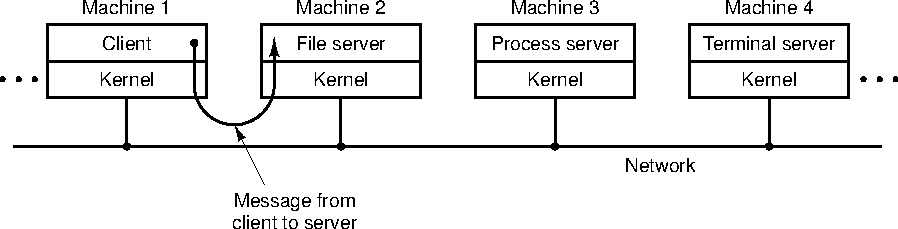
\includegraphics{fig1-27}
\caption{The Initial Stages of the Bully Algorithm.}
\label{figure:bully}
\end{figure}

\item ({\bf 10 Points}) In {\em The Mythical Man Month} Frederick Brooks identifies some of the fundamental challenges
  associated with the engineering of computer software.  Answer the following questions about the concepts developed by
  Brooks.

  \begin{enumerate}
          
  \item ({\bf 6 Points}) One of the most challenging tasks associated
    with implementing a software system is managing the software
    development team.  Brooks presents several graphs that contain
    ``People'' on the horizontal axis and ``Months'' on the vertical
    one.  What does a curve on this graph look like if $\ldots$

    \begin{enumerate}

      \item ({\bf 3 Points}) $\ldots$ a task is perfectly partitionable?
    
      \item ({\bf 3 Points}) $\ldots$ a task is not partitionable at all?

    \end{enumerate}

  \item ({\bf 4 Points}) Using his experience at IBM as a foundation
    for his ideas, Brooks describes the complete evolution of a
    programming systems product.  Using a diagram with four distinct
    quadrants, please describe the full transformation of a program
    into a programming systems product.  Please make sure that your
    diagram clearly explains the cost overheads associated with this
    transformation.

  \end{enumerate}
 

\end{enumerate}

\end{document}

